\chapter{Results and Discussion}
\label{chap:results}
The Following implementation have been done on Ubuntu Linux and our objective is to implement the framework in a Linux environment and then port it to Android.

\section{Fuse File System in Linux}

To develop a filesystem, first download the FUSE source code https://github.com/libfuse/libfuse/releases  and unpack the package This creates a FUSE directory with the source code. The
contents of the fuse directory are:
\begin{itemize}
\item ./doc contains FUSE-related documentation. At this point, there is only one file, how-fuse-
works.
\item  ./kernel contains the FUSE kernel module source code .
\item  ./include contains the FUSE API headers, which  needed to create a filesystem. The only
one you need now is fuse.h.
 \item ./lib holds the source code to create the FUSE libraries to link binaries to create a filesystem.
\item ./util has the source code for the FUSE utility library.
 \item ./example, of course, contains samples for your reference, like the fusexmp.null and hello
filesystems.\\
\end{itemize}
\textbf{Build and install FUSE:}\\
1. Run the configure script from the fuse-2.2 directory: ./configure . This creates the required
makefiles, etc.\\
2. Run ./make to build the libraries, binaries, and kernel module. Check the kernel directory for
the file ./kernel/fuse.ko -- this is the kernel module file. Also check the lib directory for fuse.o,
mount.o, and helper.o.\\
3. Run ./make install to complete the installation of FUSE.\\

\textbf{Fusepy}\\
fusepy is a Python module that provides a simple interface to FUSE\_ and
MacFUSE\_. It's just one file and is implemented using ctypes.
\section{Mounting a Demo Fuse File System in Python}
\begin{figure}[h]
   \centering
   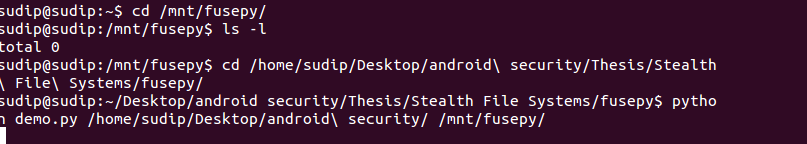
\includegraphics[width=15cm]{Figures/fig05/fusepy}
   \caption{Mounting a Fuse File System}
   
  \end{figure}
  \begin{figure}[h]
     \centering
     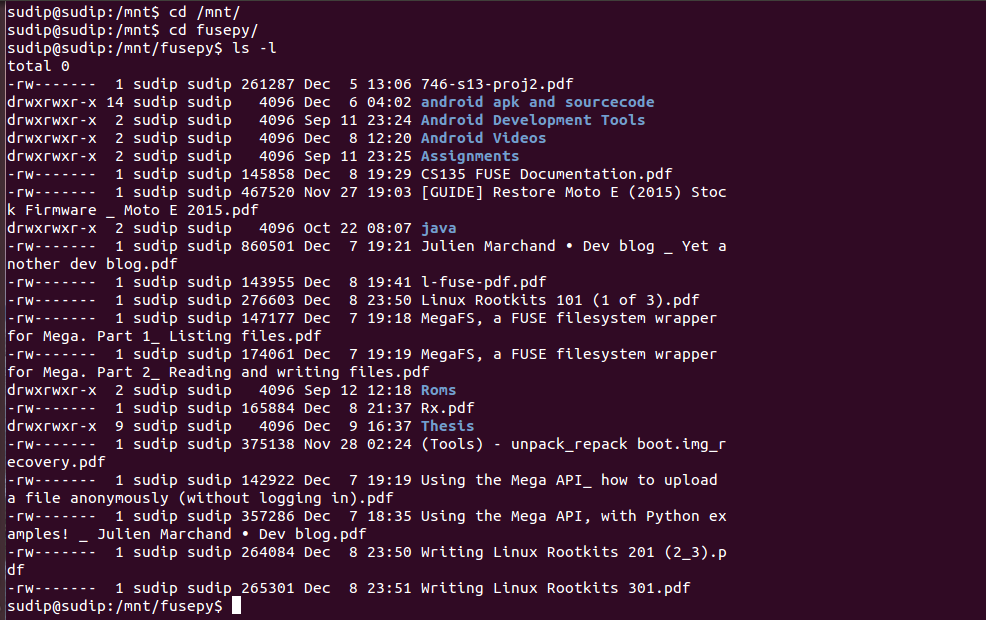
\includegraphics[width=15cm]{Figures/fig05/mnt}
     \caption{Contents of the Mounted File System}
     
    \end{figure}
    
    
\vspace{2cm}    
\section{Mounting a Cloud Drive as Local File System}



\subsection{\href{https://github.com/matteoserva/MegaFuse}{MegaFuse}}
This is a linux client for the MEGA cloud storage provider. It is based on FUSE and it allows to mount the remote cloud drive on the local filesystem. Once mounted, all linux program will see the cloud drive as a normal folder.\\

This software is based on FUSE.\\

\begin{figure}[h]
   \centering
   \textbf{Megafs.h  header Information}
   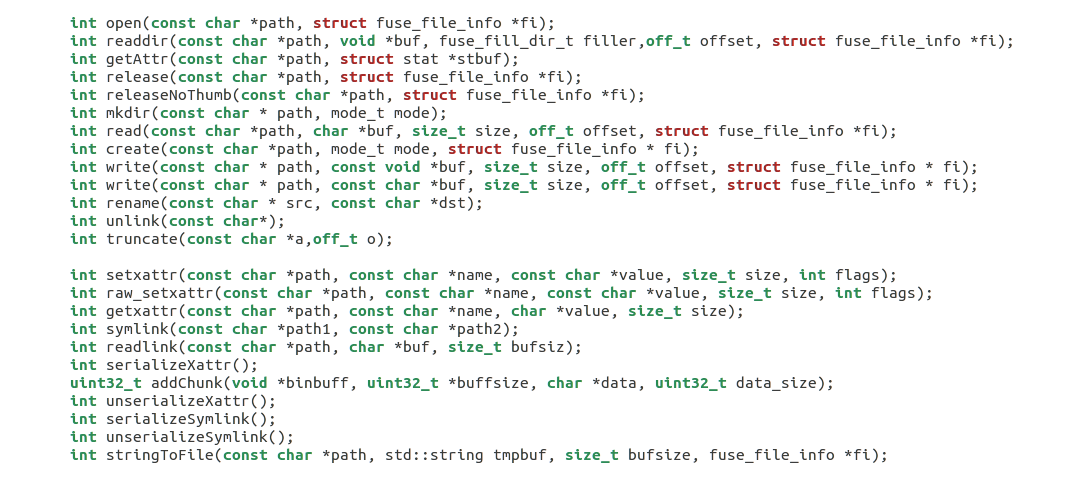
\includegraphics[width=12cm]{Figures/fig05/mega1}
   \caption{Megafuse.h defining supported  Fuse File Operations}
    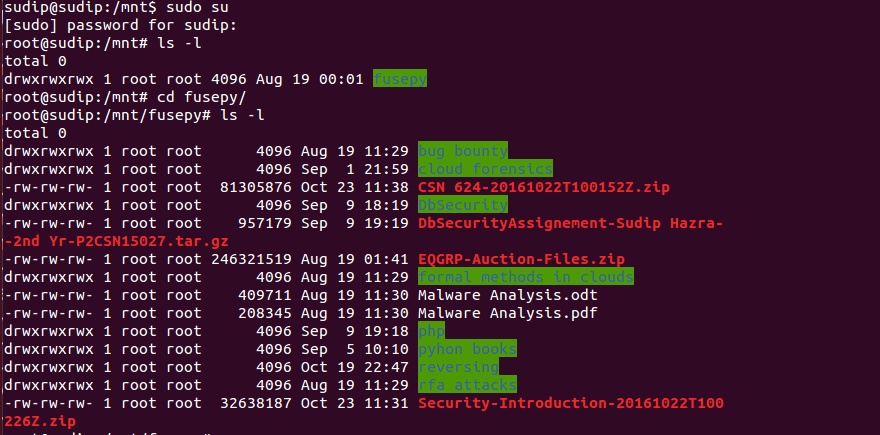
\includegraphics[width=12cm]{Figures/fig05/mega2}
                  \caption{Mounted Megafuse Cloud Drive}
   
  \end{figure}

\begin{figure}[h]
   
   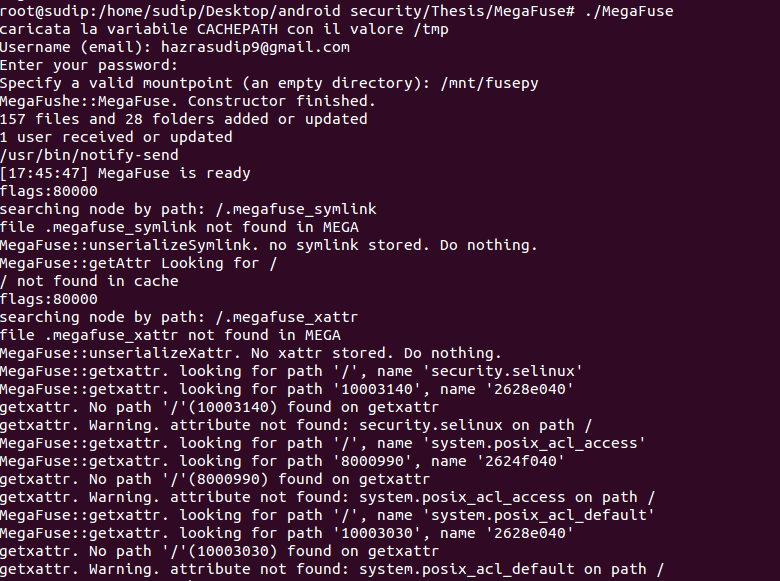
\includegraphics[width=15cm]{Figures/fig05/mega4}
   \caption{Running Megafuse Client}
   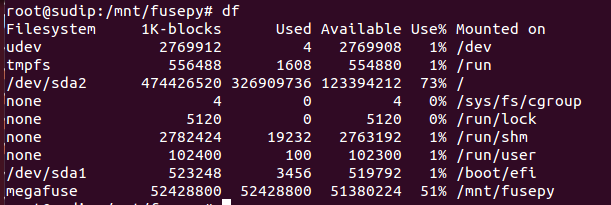
\includegraphics[width=15cm]{Figures/fig05/mega3}
        \caption{ Megafuse File System as seen by df command}
       
   
  \end{figure}

  
\section{Evidence Recovery using Sleuthkit Forensic Recovery Tool}
Sleuthkit \cite{Sleuthkit} is an open-source Forensic Recovery toolkit capable of recovering forensic artifacts from device memory image.We used an android device for 1 week and then made factory reset , and created an image of device using dd command and ran sleuthkit over it to recover artifacts.\\

\subsection{Results}
\begin{figure}[h]
   \centering
   \textbf{Running Sleuthkit Forensic Toolkit}\\
   \bigskip
   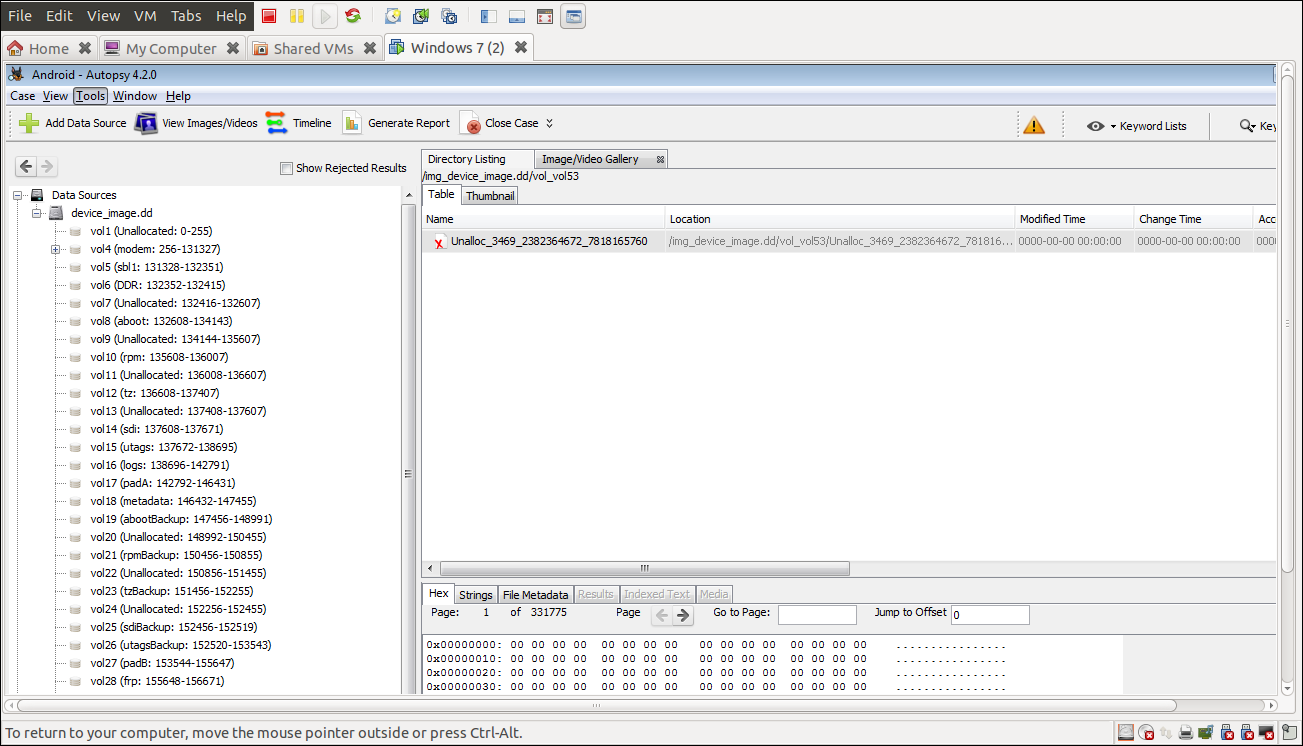
\includegraphics[width=12cm]{Figures/fig05/sleuthkit}
   \label{Sleuthkit Forensic Toolkit}
   \caption{Device image Analysis using Sleuthkit}
 \end{figure}
\begin{figure}[h]
\centering
\textbf{Recovered Images}\\
 \bigskip
  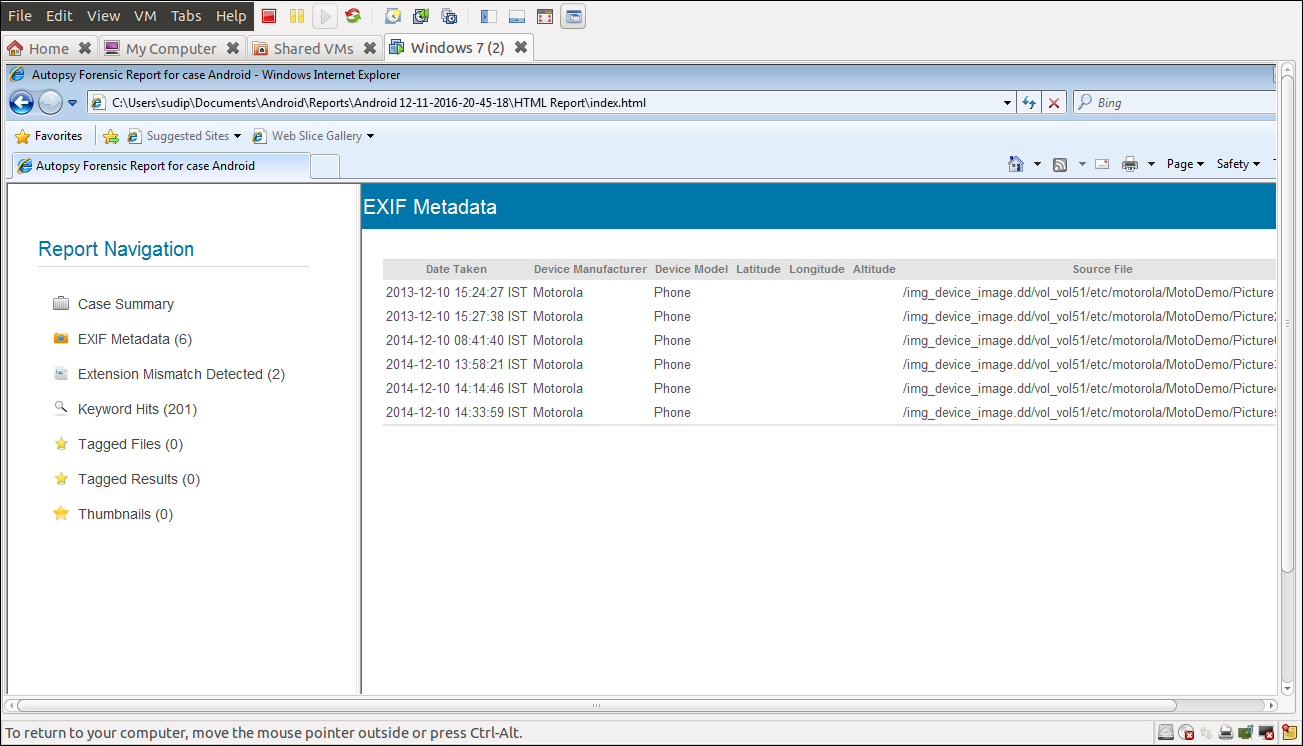
\includegraphics[width=12cm]{Figures/fig05/exitmetadata}
  
\caption[Recovered Images]{Very Few Images Could be Recovered After Factory Reset of device}
\end{figure}

\begin{figure}[h]

\centering
\textbf{Recovered Email Id's}\\
    \bigskip
    
       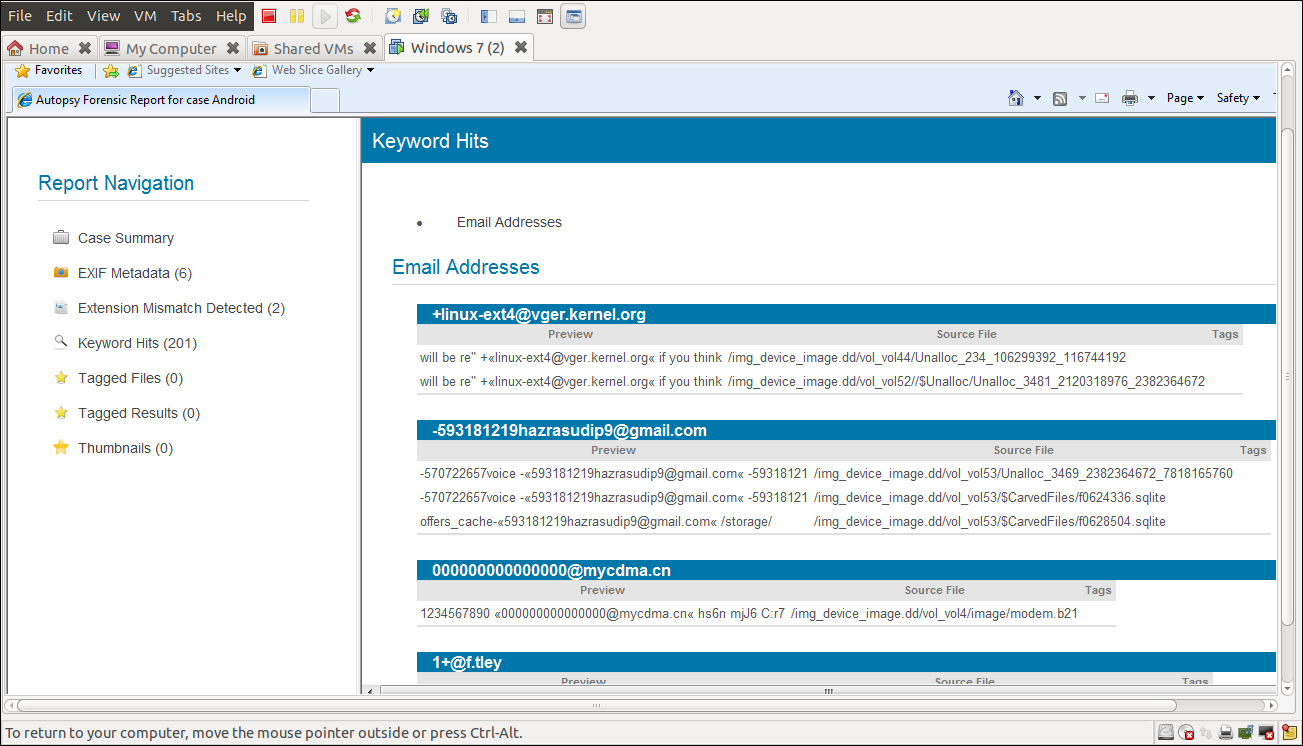
\includegraphics[width=12cm]{Figures/fig05/emails}
       \label{Email Recovery with Sleuthkit}
       \caption[Recovered Emails]{Very Few Emails Could be recovered after Factory Reset of device}
\end{figure}
\bigskip


\section{Hiding File Systems Using Rootkits}
A Rootkit can be hidden by finding out the location of the sys\_call\_table and hijack  write  with  our  own  write function. We'll first want to save a copy of the original write to pass data off to and restore when the module is unloaded.To do this we'll simply use the xchg() function and exchange the two pointers. 


\begin{figure}[h]

\centering
\textbf{Hiding Filesystems using Rootkits}\\
    \bigskip
    
       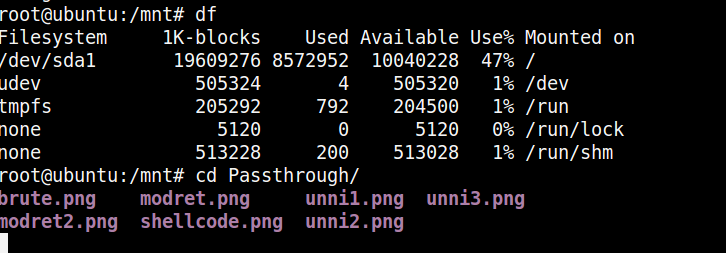
\includegraphics[width=12cm]{Figures/fig05/rooty}
       \caption[Hiding Filesystem Using Rootkits]{The write system call is highjacked, However the filesystem is still mounted.}
\end{figure}




    
 









  



